\setAuthor{Päivo Simson}
\setRound{piirkonnavoor}
\setYear{2022}
\setNumber{G 6}
\setDifficulty{6}
\setTopic{TODO}

\prob{Doomino}
\begin{wrapfigure}{r}{2.8cm}
  \vspace{-2em}
  \begin{center}
    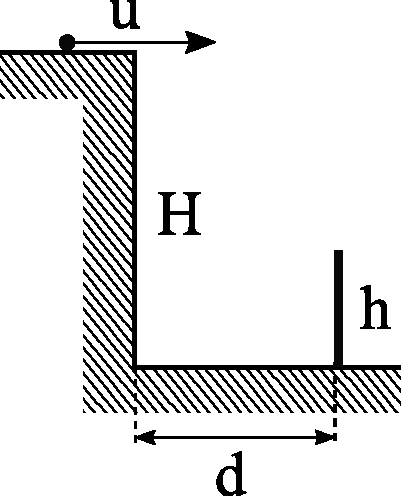
\includegraphics[width=2.8cm]{2022-v2g-06-yl.pdf}
  \end{center}
  \vspace{-2em}
\end{wrapfigure}
Väike kuulike liigub horisontaalselt kiirusega $u$ joonisel näidatud suunas ja kukub alla kõrguselt $H$. Alumisel tasapinnal on doominoklots kõrgusega $h$, mis kukub ümber, kui kuulike sellele pihta läheb. Klotsi kaugus astmest on $d$. Leidke minimaalne algkiirus $u$, mille korral kuulike teeb ühe põrke ja lendab seejärel klotsist üle. Eeldage, et õhutakistus ja hõõrdejõud puuduvad ning põrge on absoluutselt elastne. Klotsi paksusega ja kuuli mõõtmetega ei pea arvestama. Raskuskiirendus on $g$.


\hint

\solu
\begin{equation*}
\tau=\frac{d}{u}. \qquad \p1
\end{equation*}
Sellel hetkel peab kuulike olema kõrgemal kui doominoklotsi kõrgus $h$, et mitte klotsi ümber lükata. Vähimale kiirusele vastab pikim võimalik liikumise aeg \p1. On selge, et selleks peab kuulike pärast põrget uuesti tõusma kõrgusele $H$ ja seejärel langema klotsini jõudmise hetkeks mitte madalamale kui $h$ \p1. Kõrguselt $H$ kukkumise aja $t_1$ saame leida seosest $H=gt_1^2/2$, mis annab
\begin{equation*}
t_1=\sqrt{\frac{2H}{g}}. \qquad \p1
\end{equation*}
Sama aeg kulub ka pärast põrget uuesti kõrgusele $H$ tõusmiseks. Kõrguselt $H$ kõrgusele $h$ langemiseks kulub aeg
\begin{equation*}
t_2=\sqrt{\frac{2(H-h)}{g}}. \qquad \p1
\end{equation*}
Kokku kulub klotsi ülemise servani jõudmiseks aeg $2t_1+t_2=\tau=d/u$ \p1. Siit saame pärast lihtsustamist minimaalseks kiiruseks
\begin{equation*}
  u=\frac{d\sqrt{g}}{2\sqrt{2H}+\sqrt{2(H-h)}}. \qquad \p1
\end{equation*}
\probend